%

\documentclass{article}

\usepackage{fancyhdr} % Required for custom headers
\usepackage{extramarks} % Required for headers and footers
\usepackage{graphicx} % Required to insert images
\usepackage{enumerate}
\usepackage{amsmath}
\usepackage{bbold}
\usepackage{comment}

% Margins
\topmargin=-0.45in
\evensidemargin=0in
\oddsidemargin=0in
\textwidth=6.5in
\textheight=9.0in
\headsep=0.25in 

\linespread{1.1} % Line spacing

% Set up the header and footer
\pagestyle{fancy}
\lhead{Linear Algebra with Application\\
to Engineering Computation}
\chead{}
\rhead{CME 200/ME300A\\
M. Gerritsen\\
Fall 2013}
\headheight = 40pt



%th in the exponent (e.g. when writing ith, instead use i$\eth$)
\newcommand{\eth}{^{\text{th}}}


\newcommand{\R}{\mathbb{R}}

%short-cuts for Greek letters
\newcommand{\al}{\alpha}
\newcommand{\dlt}{\delta}
\newcommand{\eps}{\epsilon}

%times (cross-product)
\newcommand{\x}{\times}
%inverse
\newcommand{\inv}{^{-1}}
%cond
\newcommand{\cond}{\mathrm{cond}}
%trace
\newcommand{\trace}{\mathrm{trace}}

\newcommand{\twith}{\text{ with }}
\newcommand{\tand}{\text{ and }}
\newcommand{\tfor}{\text{ for }}
\newcommand{\tor}{\text{ or }}

\newcommand{\ip}{_{i+1}}
\newcommand{\im}{_{i-1}}

\newcommand{\half}{\frac{1}{2}}
\newcommand{\oneby}[1]{\frac{1}{#1}}
\newcommand{\overto}[1]{\overset{#1}{\longrightarrow}} 
 
\renewcommand\headrulewidth{0.4pt} % Size of the header rule
\renewcommand\footrulewidth{0.4pt} % Size of the footer rule

\setlength\parindent{0pt} % Removes all indentation from paragraphs

%----------------------------------------------------------------------------------------
%       DOCUMENT STRUCTURE COMMANDS
%       Skip this unless you know what you're doing
%----------------------------------------------------------------------------------------

% Header and footer for when a page split occurs within a problem environment
\newcommand{\enterProblemHeader}[1]{
\nobreak\extramarks{#1}{#1 continued on next page\ldots}\nobreak
\nobreak\extramarks{#1 (continued)}{#1 continued on next page\ldots}\nobreak
}

% Header and footer for when a page split occurs between problem environments
\newcommand{\exitProblemHeader}[1]{
\nobreak\extramarks{#1 (continued)}{#1 continued on next page\ldots}\nobreak
\nobreak\extramarks{#1}{}\nobreak
}

\setcounter{secnumdepth}{0} % Removes default section numbers
\newcounter{homeworkProblemCounter} % Creates a counter to keep track of the number of problems

\newcommand{\homeworkProblemName}{}
\newenvironment{homeworkProblem}[1][Problem \arabic{homeworkProblemCounter}]{ % Makes a new environment called homeworkProblem which takes 1 argument (custom name) but the default is "Problem #"
\stepcounter{homeworkProblemCounter} % Increase counter for number of problems
\renewcommand{\homeworkProblemName}{#1} % Assign \homeworkProblemName the name of the problem
\section{\homeworkProblemName} % Make a section in the document with the custom problem count
\enterProblemHeader{\homeworkProblemName} % Header and footer within the environment
}{
\exitProblemHeader{\homeworkProblemName} % Header and footer after the environment
}
\newcommand\overmat[2]{%
  \makebox[0pt][l]{$\smash{\overbrace{\phantom{%
    \begin{matrix}#2\end{matrix}}}^{\text{$#1$}}}$}#2}

\newcommand{\problemAnswer}[1]{ % Defines the problem answer command with the content as the only argument
\noindent\framebox[\columnwidth][c]{\begin{minipage}{0.98\columnwidth}#1\end{minipage}} % Makes the box around the problem answer and puts the content inside
}

\title{Assignment 8 - Solutions}
\date{Issued: November 20, 2013}
\author{Due: December 4, in class}

%----------------------------------------------------------------------------------------

\begin{document}

\maketitle
\thispagestyle{fancy}

% Problem 1
\begin{homeworkProblem}
Consider the symmetric matrix
\[ A = \begin{bmatrix} 9 & -7 \\ -7 & 17 \end{bmatrix} \]
\begin{enumerate}[(a)]
\item Compute the eigenvalues and eigenvectors of $A$.
\item Show that the eigenvectors of $A$ are orthogonal.
\end{enumerate}
\end{homeworkProblem}

\textbf{Solution:} 
\begin{enumerate}[(a)]

% Problem 1 (a)
\item The characteristic polynomial is
\[p(\lambda) = \det(A - \lambda I) = \lambda^2 - 26 \lambda + 104.\]
Solving $p(\lambda) = 0$ for $\lambda$, the eigenvalues are
\[\lambda_1 = \frac{-26 + \sqrt{26^2 - 4\x104}}{2} = 21.062, \ \ \lambda_2 = \frac{-26 - \sqrt{26^2 - 4\x104}}{2} = 4.938 \]
Solving $(A - \lambda_i I)\vec{v}_i = \vec{0}$ for $\vec{v}_i$, $i = 1,2$, the eigenvectors are
\[\vec{v}_1 = \begin{bmatrix} 1 \\ \frac{9 - \lambda_1}{7} \end{bmatrix} = \begin{bmatrix} 1 \\ -1.7232 \end{bmatrix}, \ \ \vec{v}_2 = \begin{bmatrix} 1 \\ \frac{9 - \lambda_2}{7} \end{bmatrix} = \begin{bmatrix} 1 \\ 0.5803 \end{bmatrix}\]
The normalized eigenvectors (normalized so that $\|v_i\|_2 = 1$) are
\[ \vec{v}_1 = \begin{bmatrix} 0.5019 \\ -0.8649 \end{bmatrix}, \ \ \vec{v}_2 = \begin{bmatrix} 0.8649 \\ 0.5019 \end{bmatrix}\]

% Problem 1 (b)
\item \[\vec{v}_1^T \vec{v}_2 = (0.5019 \x 0.8649) + (-0.8649 \x 0.5019) = 0\]
\end{enumerate}


% Problem 2
\begin{homeworkProblem} 
True or False? If true, prove the statement. If false, you need only provide a counterexample.
\begin{enumerate}[(a)]
\item If the $n \x n$ matrix $B$ is formed from the $n \x n$ matrix $A$ by swapping two rows of $A$, then $B$ and $A$ have the same eigenvalues.
\item Any invertible $n \x n$ matrix $A$ can be diagonalized.
\item A singular matrix must have repeated eigenvalues.
\item If the $n \x n$ matrices $A$ and $B$ are diagonalizable, so is the matrix $AB$.
\item Let $A$ be an $n \x n$ matrix. 
      \begin{enumerate}[(i)]
        \item The eigenvalues of $A$ and $A^T$ are the same.
        \item The eigenvalues and eigenvectors of $A^TA$ and $AA^T$ are the same.
      \end{enumerate}
\end{enumerate}
\end{homeworkProblem}

\textbf{Solution:}
\begin{enumerate}[(a)]

% Problem 2 (a)
\item {\bf False.} Consider
\[ A = \begin{bmatrix} 1 & 0 \\ 0 & 2 \end{bmatrix}, \tand B = \begin{bmatrix} 0 & 2 \\ 1 & 0 \end{bmatrix}\]
The eigenvalues of $A$ are 1 and 2, but the eigenvalues of $B$ are $\sqrt{2} \tand -\sqrt{2}$.

% Problem 2 (b)
\item {\bf False.} Consider
\[ A = \begin{bmatrix} 1 & 1 \\ 0 & 1 \end{bmatrix}\]
$\det(A) = 1$, so $A$ is invertible. The eigenvalues of $A$ are $\lambda_1 = \lambda_2 = 1$; the corresponding eigenvectors $\vec{v}$ must satisfy $(A - 1I) \vec{v} = \vec{0}$, or 
\[\begin{bmatrix} 0 & 1 \\ 0 & 0 \end{bmatrix} \vec{v} = \vec{0}\]
Since the matrix is upper triangular, we see by inspection that its column space has exactly one basis vector, as does its null space. Since the null space of $A - 1I$ has only one basis vector, $A$ has only one eigenvector, and therefore is not diagonalizable.

% Problem 2 (c)
\item {\bf False.}
\[ A = Y \begin{bmatrix} 1 & 0 \\ 0 & 0 \end{bmatrix}Y^{-1}\]
The eigenvector matrix can be any invertible $2 \x 2$ matrix and $A$ will be singular, but not have repeated eigenvalues.

% Problem 2 (d)
\item {\bf False.} Consider the two diagonalizable matrices (they have distinct eigenvalues)
\[ A = \begin{bmatrix} 1 & 0 \\ 0 & -1 \end{bmatrix}, \ \ B = \begin{bmatrix} 1 & 1 \\ 0 & -1 \end{bmatrix}.\]
Multiplication gives
\[ AB = \begin{bmatrix} 1 & 1 \\ 0 & 1 \end{bmatrix}, \]
which is not diagonalizable as shown in part (b)

% Problem 2 (e)
\item 
\begin{enumerate}[(i)]
  \item {\bf True.} Suppose $\lambda$ is an eigenvalue for $A$, then we have 
  \[ 0 = \det(A - \lambda I) = \det((A - \lambda I)^T) = \det(A^T - \lambda I),\]
and thus $\lambda$ is an eigenvalue for $A^T$. The converse is shown by reversing the steps above. 

  \item {\bf False.} If two matrices have the same eigenvectors and eigenvalues, then they are the same matrix. But a matrix $A$ that satisfies $AA^T = A^TA$ is called ``normal'' and not all matrices are ``normal''. Here is some matlab code to illustrate this:

\begin{verbatim}
A = rand(2)
[v1,d1]=eig(A'*A)
[v2,d2]=eig(A*A')

A =
     0.8147     0.1270
     0.9058     0.9134
v1 = 
     0.5821    -0.8131
    -0.8131    -0.5821
d1 =
     0.1840          0
          0     2.1506
v2 = 
    -0.8648     0.5021
     0.5021     0.8648
d2 = 
     0.1840          0
          0     2.1506
\end{verbatim}
\end{enumerate}
\end{enumerate}


% Problem 3
\begin{homeworkProblem}
A rabbit population $r$ and a wolf population $w$ are related according to the following system of differential equations:
\begin{eqnarray*}
\frac{dr}{dt} &=& 5r - 2w \\
\frac{dw}{dt} &=& r + 2w
\end{eqnarray*}
Here $t$ denotes time.
\begin{enumerate}[(a)]
\item If initially (at $t = 0$) there were 100 rabbits and 50 wolves, find the numbers of rabbits and wolves as a function of time $t$.
\item Design a matrix $A$ for the above system such that the populations coverge to a finite non-zero limit as $t$ goes to infinity.
\end{enumerate}
\end{homeworkProblem}

\textbf{Solution:}
\begin{enumerate}[(a)]

% Problem 3 (a)
\item If we write $\vec{x}(t) = \begin{bmatrix} r(t) \\ w(t) \end{bmatrix}$, then the system can be written as 
\[ \frac{d}{dt}\vec{x}(t) = \begin{bmatrix} 5 & -2 \\ 1 & 2 \end{bmatrix} = A\vec{x}(t).\]
We know that the solution to this system is given by $\vec{x}(t) = e^{At}\vec{x}_0$. By solving the characteristic polynomial $\det(A - \lambda I) = 0$, we find that the eigenvalues of $A$ are $\lambda_1 = 4, \lambda_2 = 3$ with corresponding eigenvectors $\vec{v}_1 = \begin{bmatrix} 2 \\ 1 \end{bmatrix}, \vec{v}_2 = \begin{bmatrix} 1 \\ 1 \end{bmatrix}$. Using the diagonalization $A = Y\Lambda Y^{-1}$, we have
\begin{align*}
\vec{x}(t) &= e^{At}\vec{x}_0 \\
&= Ye^{\Lambda t}Y^{-1}\vec{x}_0 \\
&= \begin{bmatrix} 2 & 1 \\ 1 & 1 \end{bmatrix} \begin{bmatrix} e^{4t} & 0 \\ 0 & e^{3t} \end{bmatrix} \begin{bmatrix} 2 & 1 \\ 1 & 1 \end{bmatrix}^{-1} \begin{bmatrix} 100 \\ 50 \end{bmatrix} \\
&= \begin{bmatrix} 2e^{4t} - e^{3t} & -2e^{4t} + 2e^{3t} \\ e^{4t} - e^{3t} & -e^{4t} + 2e^{3t} \end{bmatrix} \begin{bmatrix} 100 \\ 50 \end{bmatrix} \\
&= \begin{bmatrix} 100e^{4t} \\ 50e^{4t} \end{bmatrix}
\end{align*}

% Problem 3 (b)
\item There are many choices of coefficients that result in a steady equilibrium population. In general, a coefficient matrix $A$ with one zero and one negative eigenvalue will result in convergence to a non-zero equilibrium. one such matrix is 
\[ A = \begin{bmatrix} 1 & -6 \\ 1 & -6 \end{bmatrix},\]
which produce the solution
\[ \vec{x}(t) = \begin{bmatrix} 60 + 40 e^{-5t} \\ 10 + 40 e^{-5t} \end{bmatrix},\]
which approaches $\begin{bmatrix} 60 \\ 10 \end{bmatrix}$ as $t \to \infty$.
\end{enumerate}


% Problem 4
\begin{homeworkProblem}
Heat Equation. We look at the matrix
\[A = \begin{bmatrix} -2 & 1 & 0 \\ 1 & -2 & 1 \\ 0 & 1 & -2 \end{bmatrix} \]
\begin{enumerate}[(a)]

% Problem 4 (a)
\item Find the eigenvalues of $A$ and the corresponding eigenvectors. $A$ is symmetric, so the eigenvectors should be orthogonal. Check that this is the case. 

% Problem 4 (b)
\item Give the algorithm of the power method that can be used to find the largest eigenvalue (in absolute value) of $A$. 

% Problem 4 (c)
\item Execute this algorithm, either by hand or with matlab. As initial vector take one of the unit vectors. Produce a figure showing the computed approximations as a function of iteration step. Repeat with an initial vector equal to an eigenvector corresponding to either of the two smallest eigenvalues. Observe that the algorithm still converges. but slower than before (round-off error accumulation helps in this case as we discussed in class). \\ \\
Note: The matrix is well-conditioned and the round-off error will not accumulate particularly fast. Make sure you force the iteration to run for a while (we have found at least 60 iterations works) because you are only testing the relative error in successive iterates of the eigenvalues.

% Problem 4 (d)
\item Instead of looking at this $3 \x 3$ matrix, take $10 \x 10$ (or larger if you like) matrix with the same tridiagonal structure ($-2$ on the main diagonal and $1$ on the subdiagonals). Find all eigenvalues of this larger matrix using the $QR$ iterations. Check your answers against the eigenvalues computed by matlab using the \texttt{eig} command. Again, motivate your convergence criterion. 

% Problem 4 (f)
\item Since the heat equation discretization was an example of numerically solving a differential equation, the plotting of solutions was rather important. Since we just computed eigenvectors, we might be interested to see what the eigenvectors look like when plotted. Consider $102 \x 102$ discretization for the heat equation so that the matrix $A$ is $100 \x 100$. Use the \texttt{eig} command in matlab to obtain the eigenvectors $\vec{v}^{(1)}, \ldots, \vec{v}^{(100)}$ for $-A$ (this is $-A$ so there are positive 2s on the diagonal). For $j = 1, \ldots, 5$, plot $\sqrt{101}\vec{v}^{(j)}$ as we have done in previous homeworks (remember the boundary values). \\ \\
Now verify for yourself that the functions $u_j(t) = \sqrt{2}\sin (j\pi t)$ for $j = 1, 2, 3, \ldots$ satisfy the differential equation, 
\[ -\frac{d^2u_j}{dt^2} = \lambda u_j, \ \ \lambda = (j \pi)^2, \ \ u_j(0) = u_j(1) = 0, \ \ \int_0^1 u_j(t)^2 dt = 1.\]
How do the eigenvectors $\vec{v}^{(j)}$ of $-A$ compare to the ``eigenfunctions'' $u_j(t)$ of the differential equation? What significance does the factor $\sqrt{101}$ have when plotting $\sqrt{101}\vec{v}^{(j)}$ (think about a Riemann sum approximation of the above integral)?
\end{enumerate}
\end{homeworkProblem}

\textbf{Solution:}
\begin{enumerate}[(a)]
\item Using the following code we find the eigenvalues $d$ eigenvectors $v$ and check that the inner product  between the different eigenvectors are $0$.

\begin{verbatim}
n=3;
A = -2*diag(ones(n,1)) + diag(ones(n-1,1),-1) + diag(ones(n-1,1),1); 
[v,d] = eig(A)
v*v'
\end{verbatim}

\begin{verbatim}

v =

    0.5000   -0.7071   -0.5000
   -0.7071    0.0000   -0.7071
    0.5000    0.7071   -0.5000


d =

   -3.4142         0         0
         0   -2.0000         0
         0         0   -0.5858


ans =

    1.0000    0.0000    0.0000
    0.0000    1.0000    0.0000
    0.0000    0.0000    1.0000
\end{verbatim}

\item  \begin{enumerate}[(i)]

\item k = 0 : Set $v_0$ so that $\|v_0 \| = 1$ and $\lambda_0$ to an arbitrary quantity.
\item Compute $v_{k+1} = \frac{A v_k}{ \| av_k\|_2}$ and $\lambda_{k+1}  = v_k^T A v_k$.
\item If $\frac{|\lambda_{k+1} - \lambda_k| }{|\lambda_k|} < \epsilon$, stop. Otherwise repeat step 2.
  \end{enumerate}
  
  
\item The following code can be used

\begin{verbatim}
A = -2*diag(ones(3,1)) + diag(ones(2,1),-1) + diag(ones(2,1),1);
[v,d] = eig(A); d=diag(d);
v1 = v(:,2); v2 = A*v1;
lam1 = 1; lam2 = v1�*v2;
v2 = v2/norm(v2);
err = abs(lam2-lam1)/abs(lam1);
i=1;
while abs(lam2-lam1)/abs(lam1) > 10^-6 || i<60
v1 = v2; v2 = A*v1;
lam1 = lam2; lam2 = v1�*v2;
v2 = v2/norm(v2);
i=i+1;
err(i) = abs(lam2-lam1)/abs(lam1);
end
\end{verbatim}
  

The algorithm takes 83 iterations to converge to $\lambda_{max} = 3.4142$. With an relative error tolerance of $10^{-6}$, the roundoff error takes a minimum of 58 iterations to accumulate so that the algorithm can then run on its own without being forced to continue.
\\

Starting with the third eigenvector only takes 27 iterations to converge.
\\
Forcing the iteration to continue seems rather arbitrary. It is also exploiting knowledge about the problem. A better way to generate convergence is via a perturbation of the eigenvector. Convergence to one of the minor eigenvectors is not stable so if we detect convergence, we should perturb our solution vector and see if we come back to the equilibrium. This would to prevent us from having to wait for roundoff error to work in our favor. This problem was really to just see how roundoff error can work in our favor.
  
  
 \item 
 
 The QR iteration:
 \begin{verbatim}
function [A,k] = qrmeth(A)
      k = 1;  %initialize counter
      tol = 1e-5;
              %set tolerance
      while 1<3
         [Q,R] = qr(A);
         A = R*Q;
              %get the next A
         if(norm(Q*A-A*Q) < tol)
              %convergence condition is when Q*A is approx to A*Q
              %as this would mean A is approximately diagonal
             break
end
k = k+1; end
end
\end{verbatim}
 
 Applying it to our matrix:
 
 \begin{verbatim}
clear all
  close all
  m = 10; %setting dimension of A
  A = diag(-2*ones(m,1)) + diag(ones(m-1,1),1) + diag(ones(m-1,1),-1);
          %creating A
  [D,k] = qrmeth(A);
          %find e-vals of D and the number of iterations
  V = eig(A)
          %the e-vals of A using eig
  lam = diag(D)
          %extracts diagonal from D
  diff = lam-V
          %difference between these two e-vals
\end{verbatim}

The results:

\begin{verbatim}
V=
     -3.9190
     -3.6825
     -3.3097
     -2.8308
      -2.2846
     -1.7154
     -1.1692
     -0.6903
     -0.3175
     -0.0810


lam =
     -3.9190
     -3.6825
     -3.3097
     -2.8308
     -2.2846
     -1.7154
     -1.1692
     -0.6903
     -0.3175
     -0.0810
  diff =
     1.0e-07 *
      0.9251
     -0.9250
     -0.0001
      0.0000
     -0.0000
     -0.0000
     -0.0000
     -0.0000
      0.0000
     -0.0000
\end{verbatim}

\item Here are the code and plots for the eigenfunctions:

\begin{verbatim}
 n=100;
  A = -2*eye(n) + diag(ones(n-1,1),-1) + diag(ones(n-1,1),1);
  [v,d] = eig(-A);
  d = diag(d);
  t = linspace(0,1,n+2)�;
 
  k=5;
  figure
  subplot(2,1,1)
 
 
 plot(t,sqrt(n+1)*[zeros(1,k);v(:,1:k);zeros(1,k)]*diag(sign(v(1,1:k))))
title(�Discretized Eigenvectors�)
legend(�j=1�,�j=2�,�j=3�,�j=4�,j=5�);
subplot(2,1,2)
plot(t,sqrt(2)*sin(pi*t*(1:k)))
title(�ODE Eigenfunctions�)
\end{verbatim}


\begin{figure}[h!]
\centering
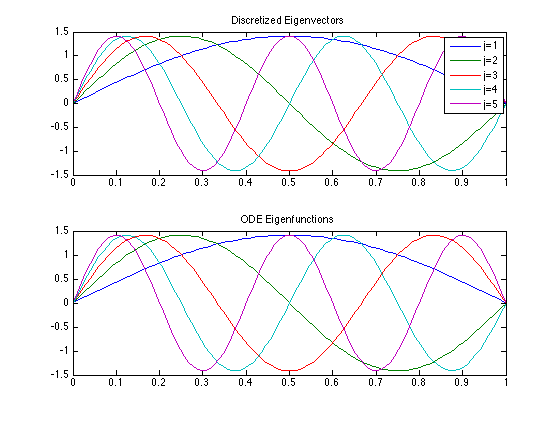
\includegraphics[ width=12cm,height=7cm]{fig1.png}
\caption{Plot of discretized and exact eigenvectors.
}
\label{fig1}
\end{figure}


The eigenvectors are discretized versions of the eigenfunctions. This makes sense because the Poisson matrix was supposed to represent a discretization of the second derivative. Note also that we have normalized the eigenvectors as $\| v_{j}\|_2 = 1$. The factor $\sqrt{101}$ serves to put the eigenvector on the same scale as the eigenfunctions:

\begin{equation*}
1 = \int_0^1 u_j(t)^2dt \approx \frac{1}{n+1} \sum_{i = 1}^{n+1} u_j(t_i)^2 \approx \frac{1}{n+1}  \sum_{i=1}^{n} (\sqrt{101}v_j(t_i))^2 = \sum_{i=1}^{n+1}  v_j(t_i)^2 = 1
\end{equation*}

  \end{enumerate}

  
% Problem 5
\begin{homeworkProblem}
In this problem we consider a small mass-spring system, consisting of 2 masses that are connected to each other and to fixed walls by three identical springs as shown in the figure. At time $t = 0$, we give the first mass $m_1$ a small displacement. As a result the mass-spring system will start to move in an oscillatory fashion. If the masses are both equal to 1, the system of equation that describes the displacement of the masses is given by 
\[ \frac{d^2\vec{u}}{dt^2} = A\vec{u}, \]
where
\[ \vec{u} = \begin{bmatrix} u_1 \\ u_2 \end{bmatrix}, \]
with $u_1 \tand u_2$ are the displacements of $m_1 \tand m_2$, respectively, and 
\[ A = \begin{bmatrix} -2 & 1 \\ 1 & -2 \end{bmatrix}. \]
We take the initial conditions (we need two of them for a second order differential equation) to be 
\[ \vec{u}(0) = \begin{bmatrix} 1 \\ 0 \end{bmatrix}, \ \ \frac{d\vec{u}}{dt}(0) = \begin{bmatrix} 0 \\ 0 \end{bmatrix}, \]

\begin{enumerate}[(a)]

% Problem 5 (a)
\item Find the matrices $Y$ and $\Lambda$ such that $A = Y \Lambda Y^{-1}$, with $Y$ orthogonal, and $\Lambda$ diagonal.

% Problem 5 (b)
\item Using this decomposition of $A$, show that we can transform the system of differential equations to
\[ \frac{d^2\vec{z}}{dt^2} = \Lambda \vec{z}, \ \ \vec{z} = Y^T \vec{u}.\]
The system for $\vec{z}$ is now ``decoupled'' so you can solve each component individually since they do not depend on each other. Solve the system of equations for $\vec{z}$ and from it find the displacements $u_1$ as a function of time $t$.

% Problem 5 (c)
\item If the masses are not equal, the system of differential equations describing the motion of the mass-spring system is instead given by 
\begin{equation} \label{mass-spring} M\frac{d^2\vec{u}}{dt^2} = A\vec{u}, \ \ M = \begin{bmatrix} m_1 & 0 \\ 0 & m_2 \end{bmatrix}.\end{equation}
We guess solution will be of the form $\vec{u}(t) = e^{i \omega t} \vec{v}$, where $\omega \tand \vec{v}$ are quantities determined by $M \tand A$. Plug in $\vec{u}(t) = e^{i \omega t} \vec{v}$ and show that finding $\omega \tand \vec{v}$ corresponds to the so-called ``generalized eigenvalue problem''
\[ A\vec{v} = \lambda M \vec{v},\]
with $\lambda = (i \omega)^2$. \\ \\
Now set $m_1 = 1$ and $m_2 = 2$. The characteristic polynomial for the generalized eigenvalue problem is given by $\det(A - \lambda M) = 0$. Solve the characteristic polynomial to find the two generalized eigenvalues $\lambda_1, \lambda_2$ (or if you wish, the two values of $\omega$ since $\lambda = (i \omega)^2$) and the two generalized eigenvectors $\vec{v}_1, \vec{v}_2$. Then give the solution to the differential equation in (\ref{mass-spring}).
\end{enumerate}
\end{homeworkProblem}

\textbf{Solution:}
  \begin{enumerate}[(a)]
\item 

\begin{equation*}
Y= \left ( \begin{array}{cc} \frac{1}{\sqrt{2}} &  \frac{1}{\sqrt{2}} \\  -\frac{1}{\sqrt{2}} &  \frac{1}{\sqrt{2}} \end{array} \right ), \qquad \Lambda= \left ( \begin{array}{cc} -3&  0 \\  0&  1\end{array} \right )
\end{equation*}

\item Let�s make the change of variables $\vec z = Y^T \vec u$. Then the ODE becomes

\begin{equation*}
\frac{d^2 \vec u}{ dt^2} = Y \Lambda \vec z.
\end{equation*}

If we pre-multiply by $Y^T$, we get  $\Lambda \vec z$ on the RHS so we have to see if in fact

\begin{equation*}
 Y^T \frac{d^2 \vec u}{ dt^2}   =  \frac{d^2  Y^T \vec u}{ dt^2} =  \frac{d^2 \vec z}{ dt^2} 
\end{equation*}





If you know multivariable calculus, this is well known to you. Otherwise, here is how the statement is verified:

\begin{equation*}
\begin{split}
& Y^T \frac{d^2 \vec u}{ dt^2} = Y^T  \left [ \begin{array}{c} \frac{d^2 \vec u_1}{ dt^2} \\ \frac{d^2 \vec u_2}{ dt^2} \end{array} \right ]  =   \left [ \begin{array}{cc} y_{11}\frac{d^2 \vec u_1}{ dt^2} & y_{21}\frac{d^2 \vec u_2}{ dt^2} \\  y_{12}\frac{d^2 \vec u_1}{ dt^2} & y_{22}\frac{d^2  \vec u_2}{ dt^2}  \end{array} \right ] \\
& =   \left [ \begin{array}{cc} y_{11}u_1(t) & y_{21}u_2(t) \\  y_{12} u_1(t) & y_{22}u_2(t)  \end{array} \right ]  =  \frac{d^2  Y^T \vec u}{ dt^2} =  \frac{d^2 \vec z}{ dt^2} 
\end{split}
\end{equation*}

With the transformed system, we now have two decoupled ODEs:

\begin{equation*}
\begin{array}{lll}
 \frac{d^2  z_1}{ dt^2} = -3z_1, & z_1(0) = \frac{1}{\sqrt{2}}, & z_1' (0)= 0, \\
 \frac{d^2  z_2}{ dt^2} = -z_1, & z_2(0) = \frac{1}{\sqrt{2}}, & z_2'(0) = 0.
\end{array}
\end{equation*}

The solutions to these ODEs give us

\begin{equation*}
\vec z = \left [\begin{array}{c}
 \frac{1}{\sqrt{2}} \cos(\sqrt{3}t) \\  \frac{1}{\sqrt{2}} \cos(t) 
\end{array} \right ]
\end{equation*}

Converting back to $\vec u$ gives


\begin{equation*}
\vec u = Y \vec z  = \left [\begin{array}{c}
 \frac{1}{2} \cos(t)  +  \frac{1}{2} \cos(\sqrt{3}t) \\  \frac{1}{2} \cos(t) -\frac{1}{2} \cos(\sqrt{3}t)
\end{array} \right ]
\end{equation*}

\item

If $\vec u =  e^{i \omega t} \vec v$, then

\begin{equation*}
e^{i\omega t} A \vec v  = M \frac{d^2 \vec u}{dt^2} = (i \omega)^2 e^{i \omega t} M \vec v.
\end{equation*}

With $\lambda = (i \omega)^2$, we divide out $e^{i \omega t}$ to get $A \vec v = \lambda M \vec v$, as desired.

For $m_1 = 1$ and $m_2 = 2$, the characteristic polynomial is

\begin{equation*}
2 \lambda^2 + 6 \lambda + 3 = 0,
\end{equation*}

with solutions $\lambda  = -\frac{3}{2} \pm \frac{\sqrt{3}}{2}$. Solving for the eigenvectors gives

\begin{equation*}
\lambda_1 = -\frac{3}{2}- \frac{\sqrt{3}}{2}, \quad \vec v_1 =  \left [\begin{array}{c} 1+ \sqrt{3} \\ -1 \end{array} \right ], \lambda_2 = -\frac{3}{2}+ \frac{\sqrt{3}}{2}, \quad \vec v_2 =  \left [\begin{array}{c} 1- \sqrt{3} \\ -1 \end{array} \right ]
\end{equation*}

We know that $\lambda = (i \omega)^2 = -\omega^2 $ which means that $\omega = \pm  \sqrt{-\lambda}$ since $\lambda$ is negative. Our solution thus has the form 

\begin{equation*}
\vec u(t) = \vec v_1 (c_1 e^{i \sqrt{-\lambda_1} t}+ c_2 e^{-i \sqrt{-\lambda_1} t}) + \vec v_2 (c_3 e^{i \sqrt{-\lambda_2} t}+ c_4 e^{-i \sqrt{-\lambda_2} t}).
\end{equation*}

If we use the initial conditions we get the conditions

\begin{equation*}
\begin{split}
& \vec u(0) = \vec v_1 (c_1 + c_2 ) + \vec v_2 (c_3 + c_4 ) = \begin{bmatrix} 1 \\ 0 \end{bmatrix},  \\
& \vec u'(0) = \vec v_1 (c_1 - c_2 ) + \vec v_2 (c_3 - c_4 ) = \begin{bmatrix} 0 \\ 0 \end{bmatrix}.
\end{split}
\end{equation*}

Since the eigenvectors are linearly independent we get from the second equation that $c_1 = c_2$ and $c_3 = c_4$. Plugging this into the first equation gives us the equation system


\begin{equation*}
 \vec u(0) = \left [ \begin{array}{cc} 1+ \sqrt{3} & 1- \sqrt{3} \\ -1 & -1 \end{array} \right ] \begin{bmatrix} c_1 \\ c_3 \end{bmatrix} = \begin{bmatrix} 1/2 \\ 0 \end{bmatrix}.
\end{equation*}

This has the solutions $c_1 = \frac{\sqrt{3}}{12}$ and $c_3 =- \frac{\sqrt{3}}{12}$. If we now use that $\cos(x) = \frac{e^{ix} + e^{-ix}}{2}$ we get that the solution is

\begin{equation*}
\begin{split}
& \vec u(t) = 2 \vec v_1 c_1 \cos(\sqrt{-\lambda_1 t}) + 2 \vec v_2 c_3 \cos(\sqrt{-\lambda_2 t})  \\
& =     \frac{\sqrt{3}}{6} \left [\begin{array}{c} 
 (1+ \sqrt{3}) \cos \left ( \left ( \frac{3}{2} + \frac{\sqrt{3}}{2} \right )t \right ) -  (1- \sqrt{3})\cos \left ( \left ( \frac{3}{2} - \frac{\sqrt{3}}{2}\right )t \right )   \\  
   \cos \left ( \left ( \frac{3}{2} - \frac{\sqrt{3}}{2} \right )t \right )  - \cos \left ( \left ( \frac{3}{2} + \frac{\sqrt{3}}{2}\right )t \right ) 
    \end{array} \right ]
    \end{split}
\end{equation*}




As a last comment we should note the following:

\begin{equation*}
A \vec v = \lambda  M \vec v \quad  \Leftrightarrow \quad M^{-1} A \vec v = \lambda \vec v.
\end{equation*}



That is, those generalized eigenvalues and eigenvectors are of the plain variety for the matrix $M^{-1}A$. Now, we don�t typically use $M^{-1}A$ because M might be difficult to invert or not even invertible, hence why mathematicians came up with the generalized eigenvalue problem. This happened to not be the case here, though. However, recognizing this equivalence we could have used our diagonalization technique from part (b) for this problem.














\begin{comment}


\begin{equation*}
\begin{split}
& M \frac{d^2 \vec u }{ dt^2} = A \vec u \\
\Rightarrow \quad  &  \frac{d^2 \vec u }{ dt^2} = M^{-1}A \vec u = V \Lambda V^{-1} \vec u \\
\Rightarrow \quad  &  \frac{d^2 \vec z }{ dt^2} =   V \Lambda   \vec z, \quad \vec z =  V^{-1} \vec u, \quad \vec z_{0} = V^{-1} \vec u_0'.
\end{split}
\end{equation*}

where $\Lambda$ and $V$ are the eigenvalue and eigenvector matrices for $M^{-1}A$ respectively, and $V$ is not orthogonal.
\\

As in part (b), we can write this as the decoupled system,

\begin{equation*}
\begin{array}{lll}
 \frac{d^2  z_1}{ dt^2} = \lambda_1 z_1, & z_1(0) = \vec w_1^T \vec u_0, & z_1' (0)= 0, \\
 \frac{d^2  z_2}{ dt^2} =\lambda_2 z_2, & z_2(0) = \vec w_2^T \vec u_0, & z_2'(0) = 0.
\end{array}
\end{equation*}

where

\begin{equation*}
V^{-1 } = \left [ \begin{array}{c} w_1^T \\ w_2^T
\end{array} \right ]
\end{equation*}

and, since $\lambda_1, \lambda_2 < 0$, leads to the solution

\begin{equation*}
\vec z = \left [ \begin{array}{c} w_1^T \vec u_0 \cos (\sqrt{|\lambda_1|t}) \\ w_2^T  \vec u_0 \cos (\sqrt{|\lambda_1|t)}.
\end{array} \right ]
\end{equation*}

Finally, we get the solution $\vec u$ by undoing the diagonalizing transformation so that

\begin{equation*}
\vec u = V \vec z =  [ w_1^T \vec u_0 \cos (\sqrt{|\lambda_1|t}) ] \vec v_1+ [w_2^T  \vec u_0 \cos (\sqrt{|\lambda_1|t}) ] \vec v_2.
\end{equation*}


Plugging in the values gives us,

\begin{equation*}
\begin{split}
& V = \left [\begin{array}{cc} 1+ \sqrt{3} & 1- \sqrt{3} \\ -1 & -1 \end{array} \right ], \quad  V^{-1} = \left [\begin{array}{cc} \frac{\sqrt{3}}{6} &  \frac{\sqrt{3}-3}{6}  \\  - \frac{\sqrt{3}}{6}  & - \frac{\sqrt{3}-3}{6}  \end{array} \right ] \\
& \vec z(0) = \left [\begin{array}{c} \frac{\sqrt{3}}{6}  \\ -\frac{\sqrt{3}}{6}  \end{array} \right ], \vec{ z'}(0) = \left [\begin{array}{c} 0 \\ 0 \end{array} \right ], \vec z(t) = \left [\begin{array}{c} \cos \left ( \frac{3}{2} + \frac{\sqrt{3}}{2}t \right )  \\   - \cos \left ( \frac{3}{2} - \frac{\sqrt{3}}{2}t \right )   \end{array} \right ]
\end{split}
\end{equation*}


and finally


\begin{equation*}
  \vec u(t) = \frac{\sqrt{3}}{6} \left [\begin{array}{c} 
 (1+ \sqrt{3}) \cos \left ( \frac{3}{2} + \frac{\sqrt{3}}{2}t \right ) -  (1- \sqrt{3})\cos \left ( \frac{3}{2} - \frac{\sqrt{3}}{2}t \right )   \\  
   \cos \left ( \frac{3}{2} - \frac{\sqrt{3}}{2}t \right )  - \cos \left ( \frac{3}{2} + \frac{\sqrt{3}}{2}t \right ) 
    \end{array} \right ]
\end{equation*}


Doing this in Matlab gives the following for $\vec u$


\begin{equation*}
  \vec u(t) =  \left [\begin{array}{c} 
0.7887\cos \left ( 1.5 + 0.8660 t \right ) -  0.2113 \cos \left ( 1.5 - 0.8660t \right )   \\  
  0.2887 \cos \left ( 1.5 - 0.8660t \right )  - 0.2887\cos \left (1.5 +0.8660t \right ) 
    \end{array} \right ].
\end{equation*}

\end{comment}

\end{enumerate}

  
  
  
  
  
  
  
  
  
  
\end{document}
 
 
 
